
\section{Versuchsdurchführung}
%

\subsection{ Allgemeiner Versuchsaufbau}

In diesem Termin wurden folgende Geräte verwendet:
%
\begin{itemize}
    \item  Digitaloszilloskop Rigol MSO1074Z
    \item einstellbarer Funktionsgenerator Tektronix AFG1022
    \item einstellbare Spannungsquelle Rigol DP832
    \item USB-Oszilloskop, einstellbare Spannungsquelle Analog Discovery 2
\end{itemize}

Im ganzen Versuch wurde als Operationsverstärker TL072 verwendet.

\begin{figure}[H]
  \centering
  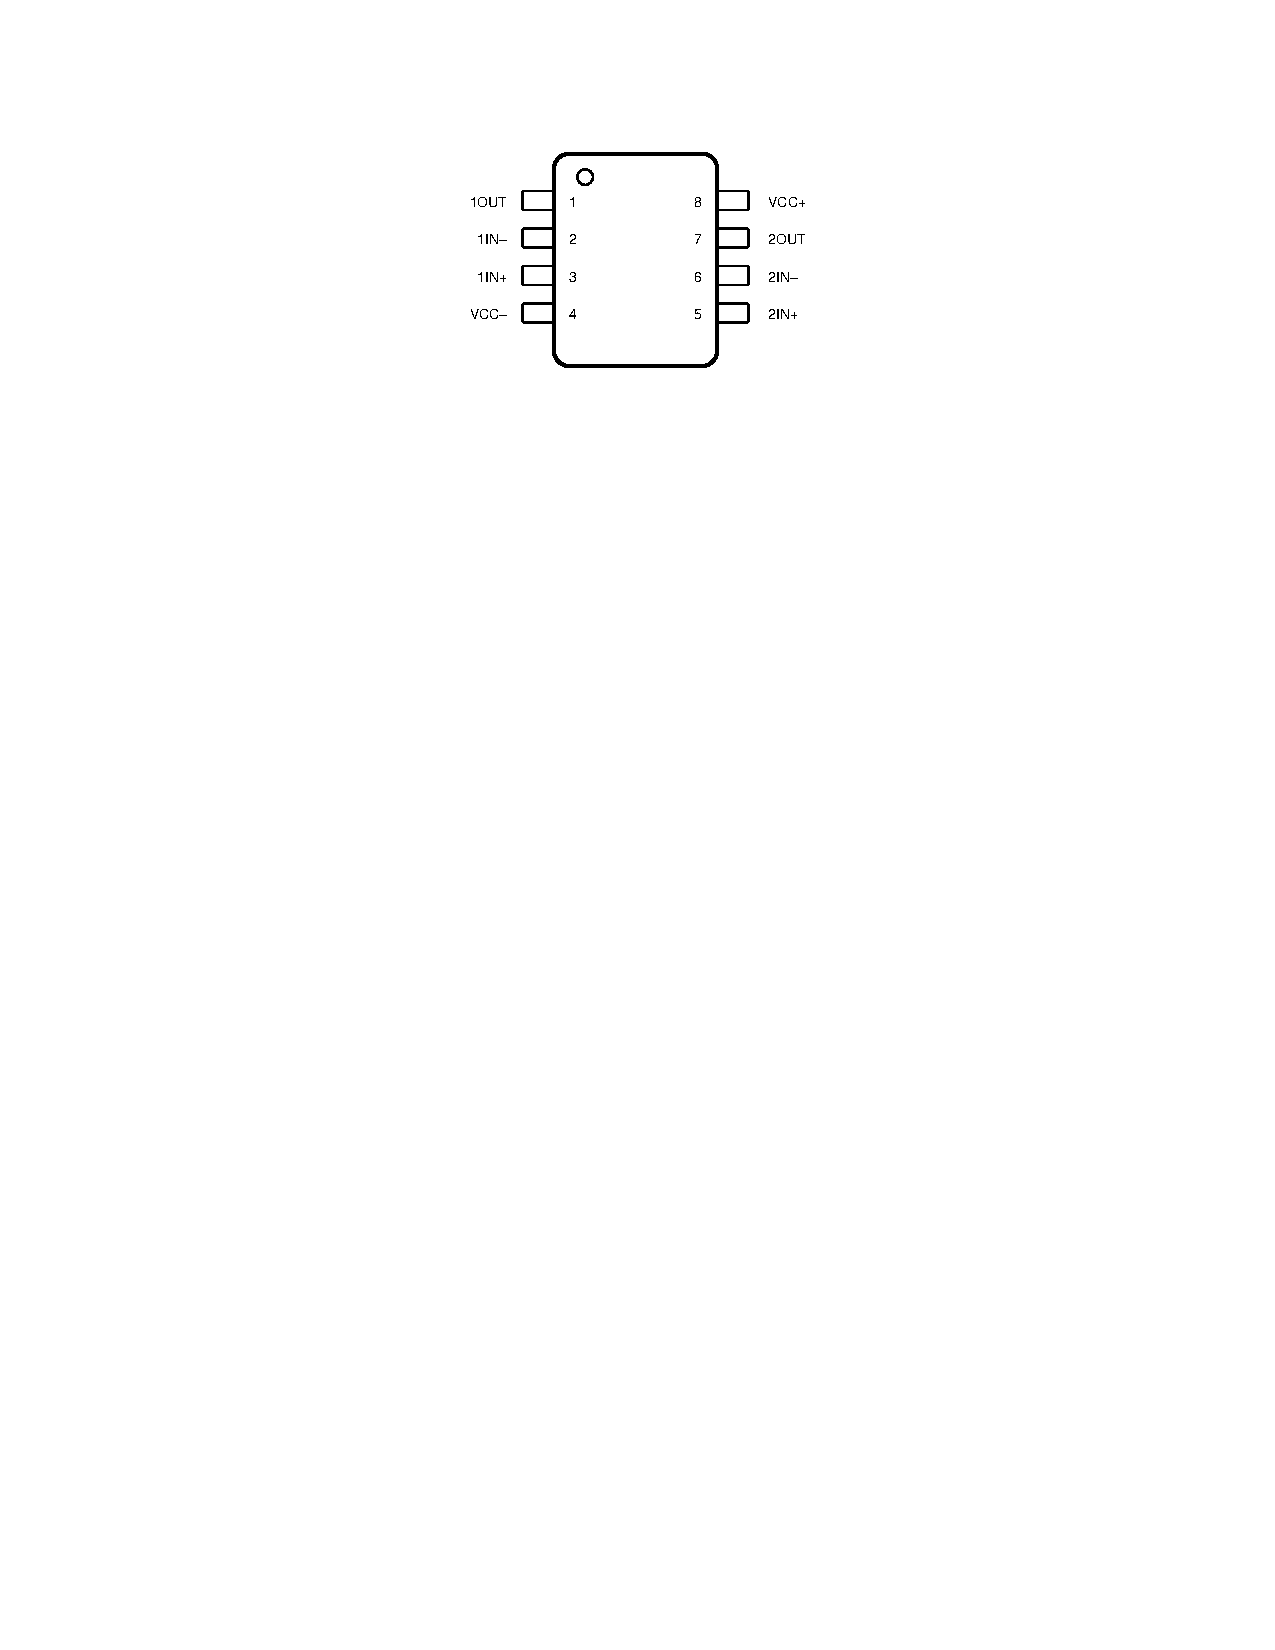
\includegraphics[width=0.4\linewidth]{Elektronik-Laborprotokoll_Filter/Abbildungen/Tl072_Datenblatt.pdf}
  \caption{TL072 \cite{Datenblatt:TL072}}
  \label{fig:Datenblatt}
\end{figure}

Bevor die Messungen in jeweiligen Teilversuchen aufgenommen wurden, wurde der Operationsverstärker von der Gleichspannungsquelle sowohl mit einer positiven als auch mit einer negativen Spannung versorgt. Die positive Versorgungsspannung beträgt \SI{12}{\volt} und die negative Versorgungsspannung beträgt \SI{-12}{\volt}.

Jede Schaltung, die auf dem Steckbrett aufgebaut wurde, wurde zusätzlich mithilfe KiCads simuliert und untersucht.

%
\subsection{Der Integrator}
%
In diesem Teilversuch wurde ein invertierender Integrator aufgebaut.
Es wurden folgende Bauteile verwendet:
%
\begin{itemize}
    \item Operationsverstärker TL072
    \item Ohmsche Widerstände mit $R_1=\SI{10}{\kilo\ohm}$ und $R_2=\SI{1}{\mega\ohm}$  %Wie groß?
    \item Kondensator mit $C=\SI{100}{\nano\farad}$
\end{itemize}
    
 Die Grundschaltung des invertierenden Integrators (Abb. \ref{fig:circuit_Integrator}) wurde mit einem hochohmigen Widerstand erweitert, damit sich die Schaltung im Betrieb auf 0 setzen lässt. Die erweiterte Schaltung (Abb. \ref{fig:circuit_Integrator_erweitert}) wurde auf dem Steckbrett aufgebaut.
 
\begin{figure}[H]
  \centering
  \begin{subfigure}{0.48\textwidth}
   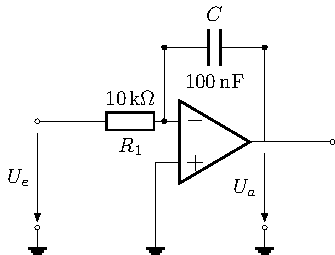
\includegraphics[width=0.7\linewidth]{Elektronik-Laborprotokoll_Filter/Circuits/Integrator.pdf}
  \caption{Grundschaltung}
    \label{fig:circuit_Integrator}
  \end{subfigure}\hfill
  \begin{subfigure}{0.48\textwidth}
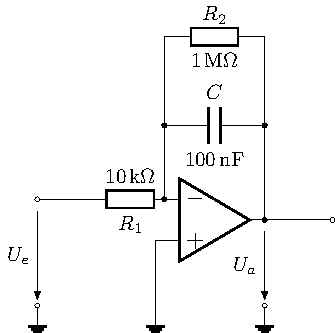
\includegraphics[width=0.7\linewidth]{Elektronik-Laborprotokoll_Filter/Circuits/Integrator_erweitert.pdf}
  \caption{erweiterte Schaltung }
  \label{fig:circuit_Integrator_erweitert}
  \end{subfigure}
  \caption{invertierender Integrator}
  \label{fig:invertierender Integrator}
\end{figure}

Die Abbildung \ref{fig:Steckbrett_Integrator} zeigt die Anordnung jeweiliger verwendeten Bauteile für die invertierende Integrator-Schaltung auf dem Steckbrett.

\begin{figure}[H]
  \centering
  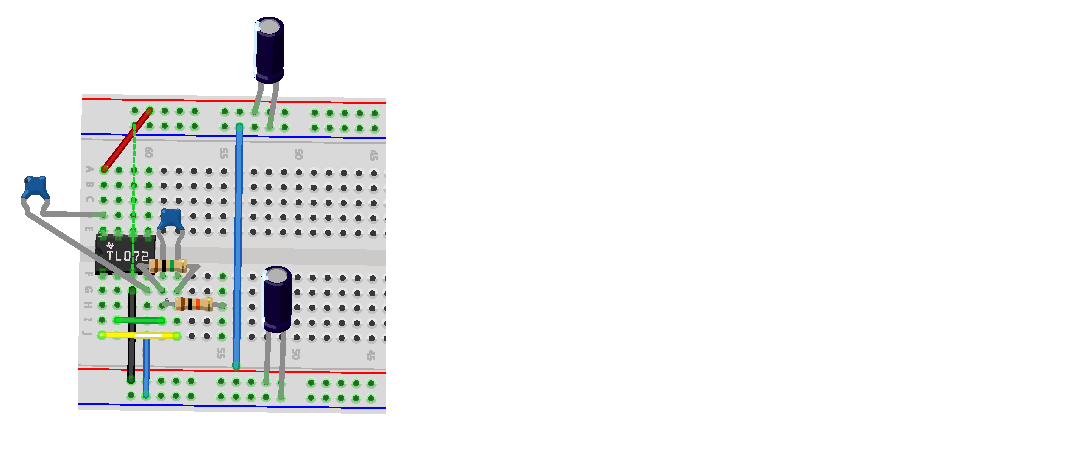
\includegraphics[width=0.4\linewidth]{Elektronik-Laborprotokoll_Filter/Abbildungen/Steckbrett_Bilder/Steckbrett_invertierender_Integrator.pdf}
  \caption{Integrator(Steckbrett)}
  \label{fig:Steckbrett_Integrator}
\end{figure}

  Der Operationsverstärker wurde von der Gleichspannungsquelle versorgt und dann wurde von dem Funktionsgenerator eine Eingangsspannung mit folgenden Eigenschaften erzeugt:
   
\begin{itemize}
    \item Form = Sinus 
    \item Frequenz = \SI{10}{\hertz}/\SI{100}{\hertz}/\SI{1000}{\hertz}/\SI{10}{\kilo\hertz}/\SI{100}{\kilo\hertz}/\SI{1}{\mega\hertz}
    \item Amplitude = \SI{500}{\milli\volt}
\end{itemize}
Zuletzt wurde es die Amplitude der Eingangspannung und der Ausgangsspannung sowie der Phasenunterschied zwischen der Ein-, und Ausgangsspannung gemessen und notiert.

    %

\subsection{Aktive Filter erster Ordnung}

In diesem Teilversuch wurde ein aktives Tiefpassfilter erster Ordnung aufgebaut.
Es wurden folgende Bauteile verwendet:
%
\begin{itemize}
\item Operationsverstärker TL072
    \item Ohmscher Widerstand mit $R_1=\SI{10}{\kilo\ohm}$ und $R_2=\SI{10}{\kilo\ohm}$
    \item Kondensator mit $C=\SI{100}{\nano\farad}$
\end{itemize}
%
Ein Tiefpassfilter mit folgender Schema \ref{fig:circuit_Tiefpass} wurde aufgebaut.


\begin{figure}[H]
  \centering
  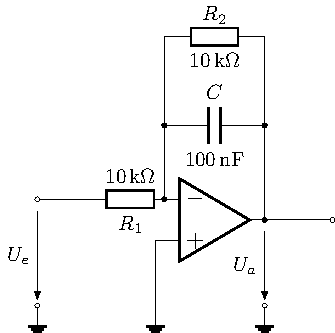
\includegraphics[width=0.4\linewidth]{Elektronik-Laborprotokoll_Filter/Circuits/Tiefpass.pdf}
  \caption{Tiefpassfilter}
  \label{fig:circuit_Tiefpass}
\end{figure}

Die Abbildung \ref{fig:Steckbrett_Tiefpass} zeigt die Anordnung jeweiliger verwendeten Bauteile des Tiefpassfilters auf dem Steckbrett.

\begin{figure}[H]
  \centering
  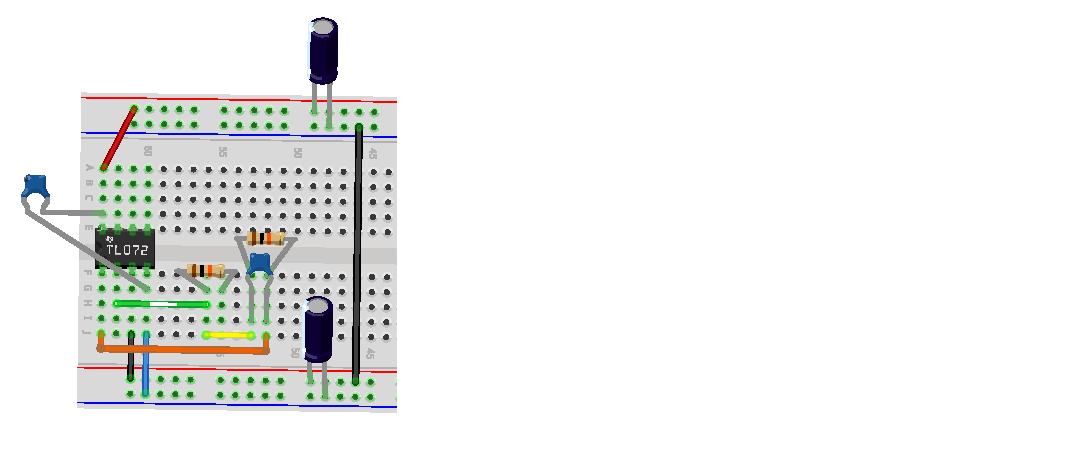
\includegraphics[width=0.5\linewidth]{Elektronik-Laborprotokoll_Filter/Abbildungen/Steckbrett_Bilder/Steckbrett_Tiefpass.pdf}
  \caption{Tiefpass(Steckbrett)}
  \label{fig:Steckbrett_Tiefpass}
\end{figure}

Erstens wurde der Operationsverstärker von der Gleichspannungsquelle versorgt. Dann wurde das vom USB-Oszilloskop/einstellbare Spannungsquelle Analog Discovery 2 das Eingangssignal erzeugt und gleichzeitig, mit der Ausgangsspannung gemessen. Das erzeugte Eingangsspannung hatte folgende Eigenschaften:
\begin{itemize}
    \item Form = Sinus 
    \item Frequenz = \SI{10}{\hertz}/\SI{100}{\hertz}/\SI{160}{\hertz}/\SI{1000}{\hertz}/\SI{10}{\kilo\hertz}/\SI{100}{\kilo\hertz}/\SI{500}{\kilo\hertz}
    \item Amplitude = \SI{500}{\milli\volt}
\end{itemize}
    Danach wurden die gemessenen Messwerte für die oben stehenden Frequenzen gespeichert. Zuletzt wurde die Frequenz des Eingangssignals von einer Frequenz von \SI{1}{\hertz} bis \SI{1}{\mega\hertz} kontinuierlich variiert und das Bode-Diagramm aufgenommen.
%
\subsection{PI Filter}
In diesem Teilversuch wurde ein PI Filter aufgebaut.
Es wurden folgende Bauteile verwendet:%
%
\begin{itemize}
    \item Operationsverstärker TL072
    \item Ohmscher Widerstand mit $R_1=\SI{10}{\kilo\ohm}$ und $R_2=\SI{10}{\kilo\ohm}$
    \item Kondensator mit $C=\SI{100}{\nano\farad}$
\end{itemize}

Ein PI Filter mit folgender Schema \ref{fig:PI_Filter_circuit} wurde aufgebaut.

\begin{figure}[H]
  \centering
  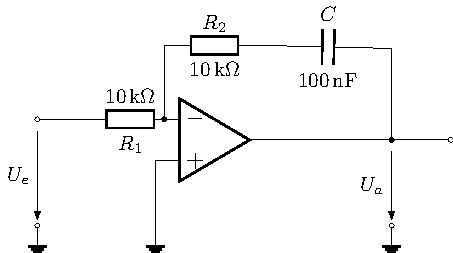
\includegraphics[width=0.5\linewidth]{Elektronik-Laborprotokoll_Filter/Circuits/PI_Filter.pdf}
  \caption{PI Filter}
  \label{fig:PI_Filter_circuit}
\end{figure}

Die Abbildung \ref{fig:Steckbrett_PI-Filter} zeigt die Anordnung jeweiliger verwendeten Bauteile des PI Filters auf dem Steckbrett.

\begin{figure}[H]
  \centering
  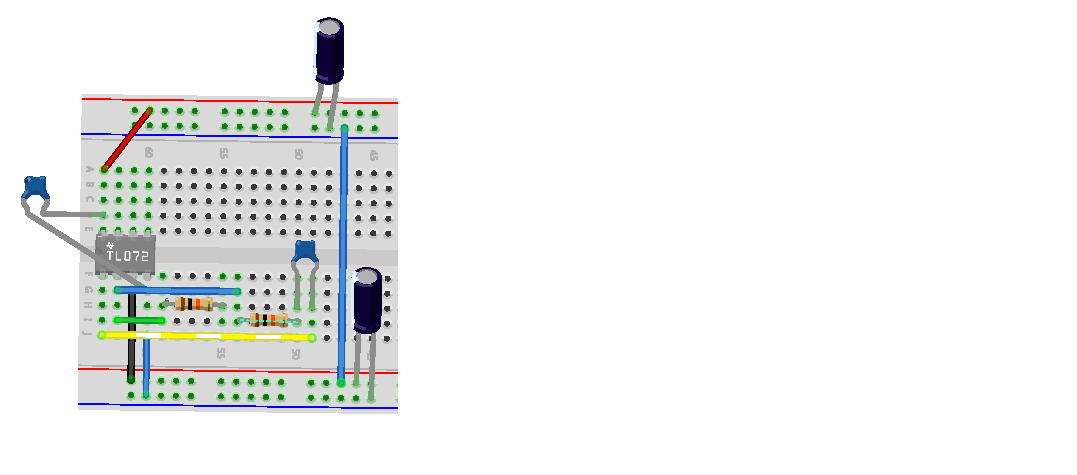
\includegraphics[width=0.4\linewidth]{Elektronik-Laborprotokoll_Filter/Abbildungen/Steckbrett_Bilder/Steckbrett_PI-Filter.pdf}
  \caption{PI Filter(Steckbrett)}
  \label{fig:Steckbrett_PI-Filter}
\end{figure}

Erstens wurde der Operationsverstärker von der Gleichspannungsquelle sowohl mit einer positiven als auch mit einer negativen Spannung versorgt und dann wurde das vom USB-Oszilloskop/einstellbare Spannungsquelle Analog Discovery 2 das Eingangssignal erzeugt und gleichzeitig, mit der Ausgangsspannung gemessen. Das erzeugte Eingangsspannung hatte folgende Eigenschaften:

\begin{itemize}
    \item Form = Sinus 
    \item Frequenz = \SI{10}{\hertz}...\SI{900}{\kilo\hertz} (101 Messwerte)
\end{itemize}
%
Mithilfe der am Eingang eingelegten Sinusspannung wurden für das Bodediagramm benötigte Messdaten aufgenommen.\\
%
Noch wurde ein anderes Eingangssignal mit folgenden Eigenschaften erzeugt:

\begin{itemize}
    \item Form = Rechteck 
    \item Frequenz = \SI{100}{\hertz}
    \item Amplitude =\SI{1}{\volt}
    \item Periodendauer = \SI{10}{\milli\second}
\end{itemize}

Die Ausgangsspannung und die Eingangsspannung wurde für die Bestimmung der Sprungantwort gespeichert.


\subsection{Sallen-Key und MFB}

In diesem Teilversuch wurde ein Sallen-Key-Filter aufgebaut. Die Bauteile wurden mithilfe des Filter Design Tool vom Texas Instruments \cite{Texas_Instruments} nach einem Tiefpassfilter 2.Ordnung (Butterworth) richtig dimensioniert.Die Konfiguration erfolgt unter Berücksichtigung der verfügbaren Widerstandswerte und Kondensatoren im Labor.

Es wurden folgende Bauteile verwendet:
%
\begin{itemize}
    \item Operationsverstärker TL072
    \item Ohmsche Widerstände mit $R_1=\SI{5,6}{\kilo\ohm}$ und $R_2=\SI{8,2}{\kilo\ohm}$
    \item Kondensatoren mit $C_1=\SI{100}{\nano\farad}$ und $C_2=\SI{205}{\nano\farad}$
\end{itemize}

Der Sallen-Key-Filter mit folgender Schema \ref{fig:Sallenkey_circuit} wurde aufgebaut.

\begin{figure}[H]
  \centering
  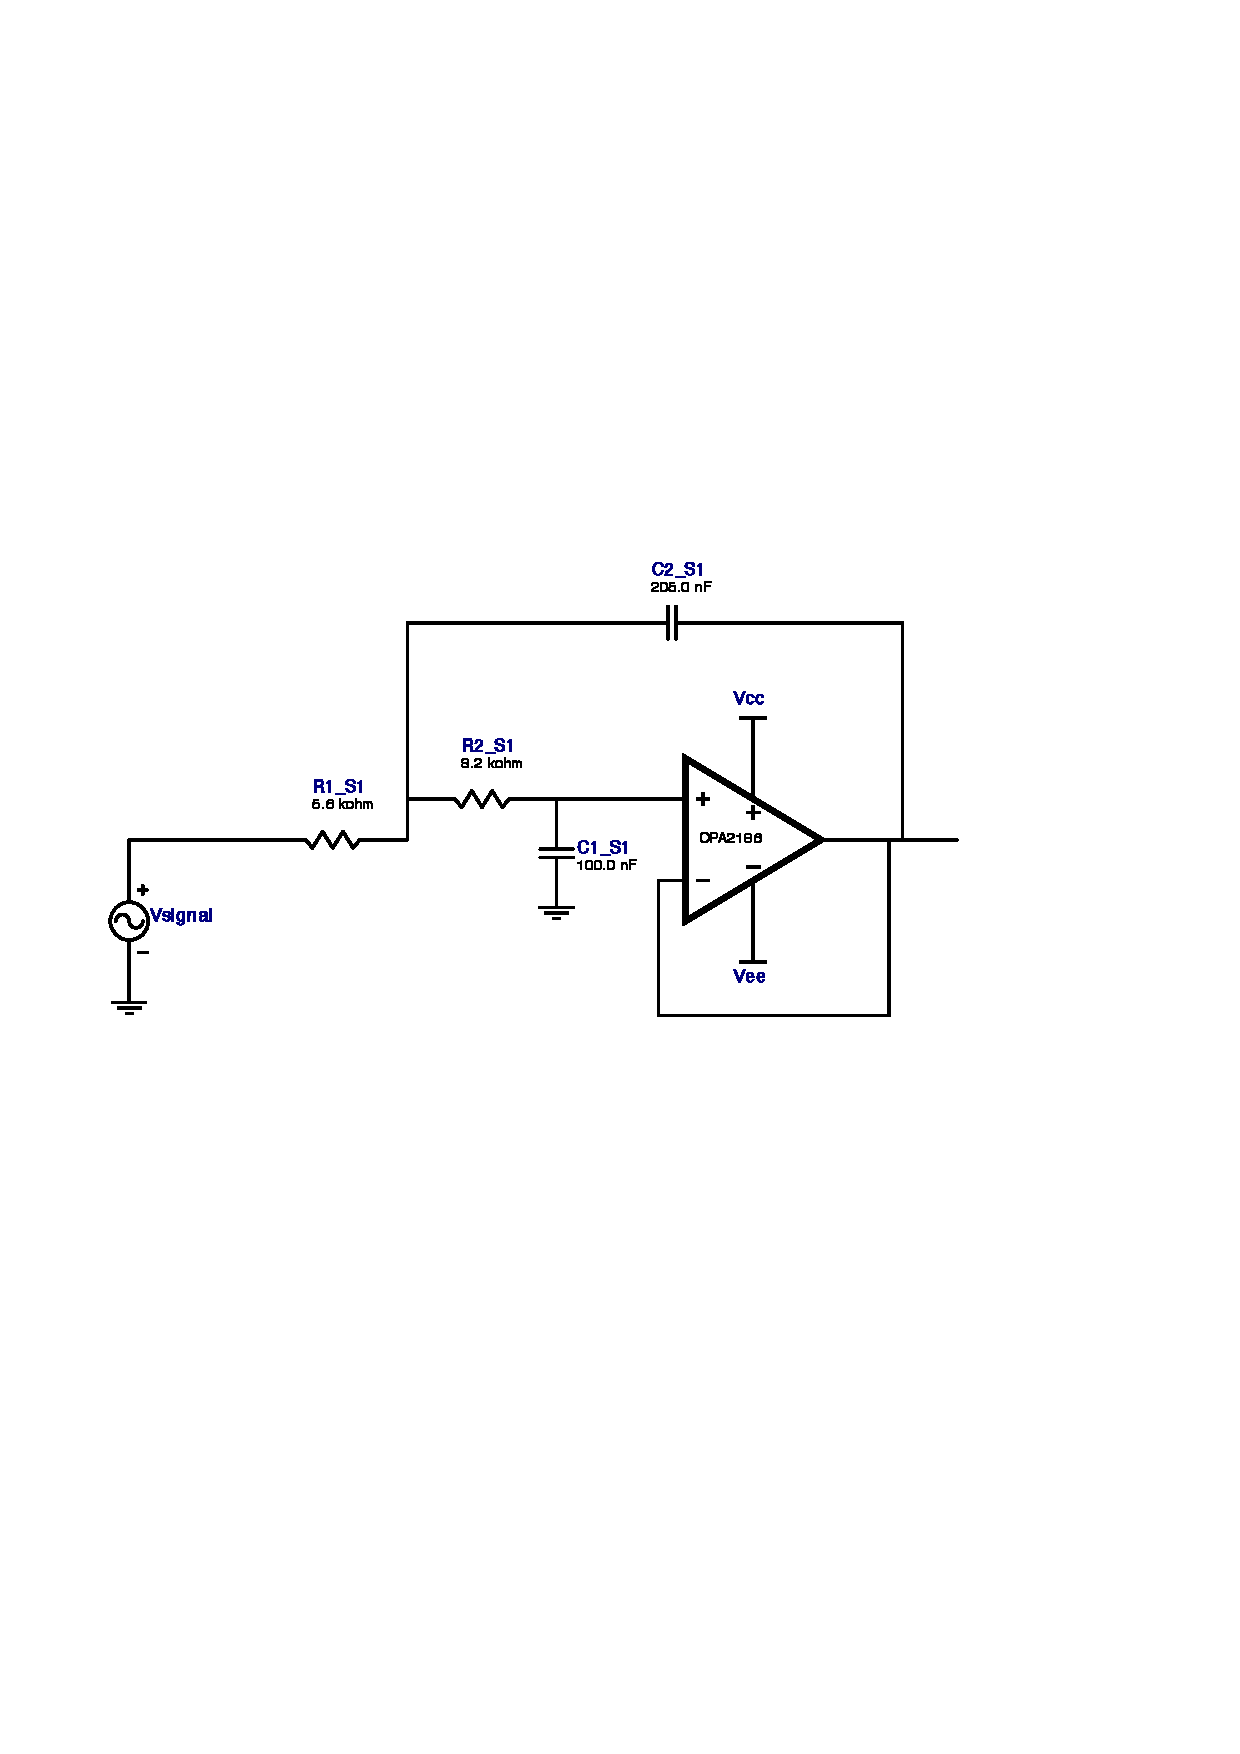
\includegraphics[width=0.5\linewidth]{Elektronik-Laborprotokoll_Filter/Circuits/SallenKey_Design.pdf}
  \caption{Sallen-Key Filter}
  \label{fig:Sallenkey_circuit}
\end{figure}

Es wurde vom USB-Oszilloskop/einstellbare Spannungsquelle Analog Discovery 2 das Eingangssignal erzeugt und gleichzeitig, mit der Ausgangsspannung gemessen. Das erzeugte Eingangsspannung hatte folgende Eigenschaften:

\begin{itemize}
    \item Form = Sinus 
    \item Frequenz = \SI{10}{\hertz}...\SI{900}{\kilo\hertz} (101 Messwerte)
\end{itemize}
%
Mithilfe der am Eingang eingelegten Sinusspannung wurden für das Bodediagramm benötigte Messdaten aufgenommen.

 
%
\subsection{Universalfilter (simulativ)}

In diesem Teilversuch wurde ein Universalfilter simuliert (\ref{fig:Universal_circuit}).


\begin{figure}[H]
 \centering
 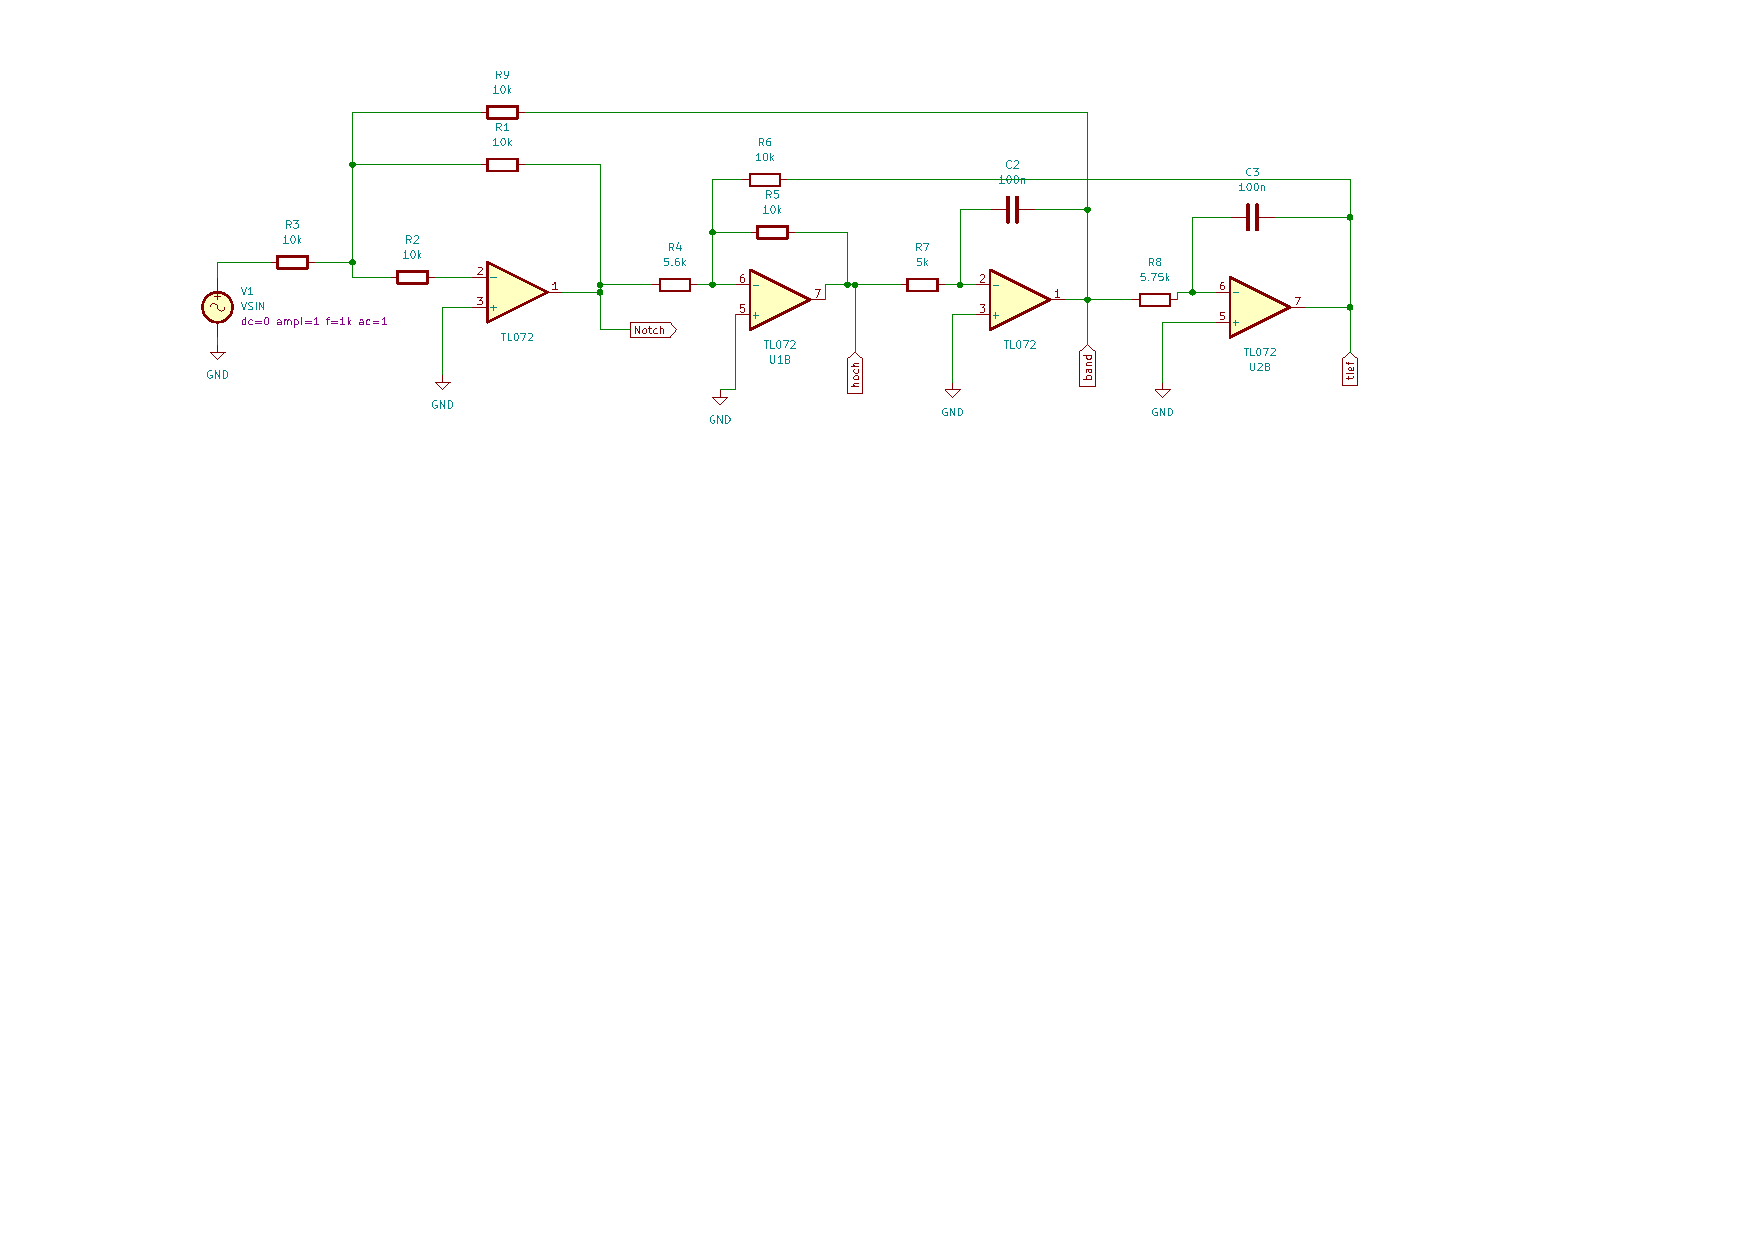
\includegraphics[width=0.7\linewidth]{Elektronik-Laborprotokoll_Filter/Circuits/universalfilter.pdf}
 \caption{ Universalfilter-Schaltung}
 \label{fig:Universal_circuit}
\end{figure}


Die Schaltung wurde in KiCad aufgebaut und mithilfe der simulierten Werte wurde ein Bodediagramm erstellt.

\subsection{Allpass und Phasenkompensatoren(simulativ)}
%
In diesem Teilversuch wurde erstens ein Allpassfilter simuliert(\ref{fig:Allpass_circuit}).
%
\begin{figure}[H]
 \centering
 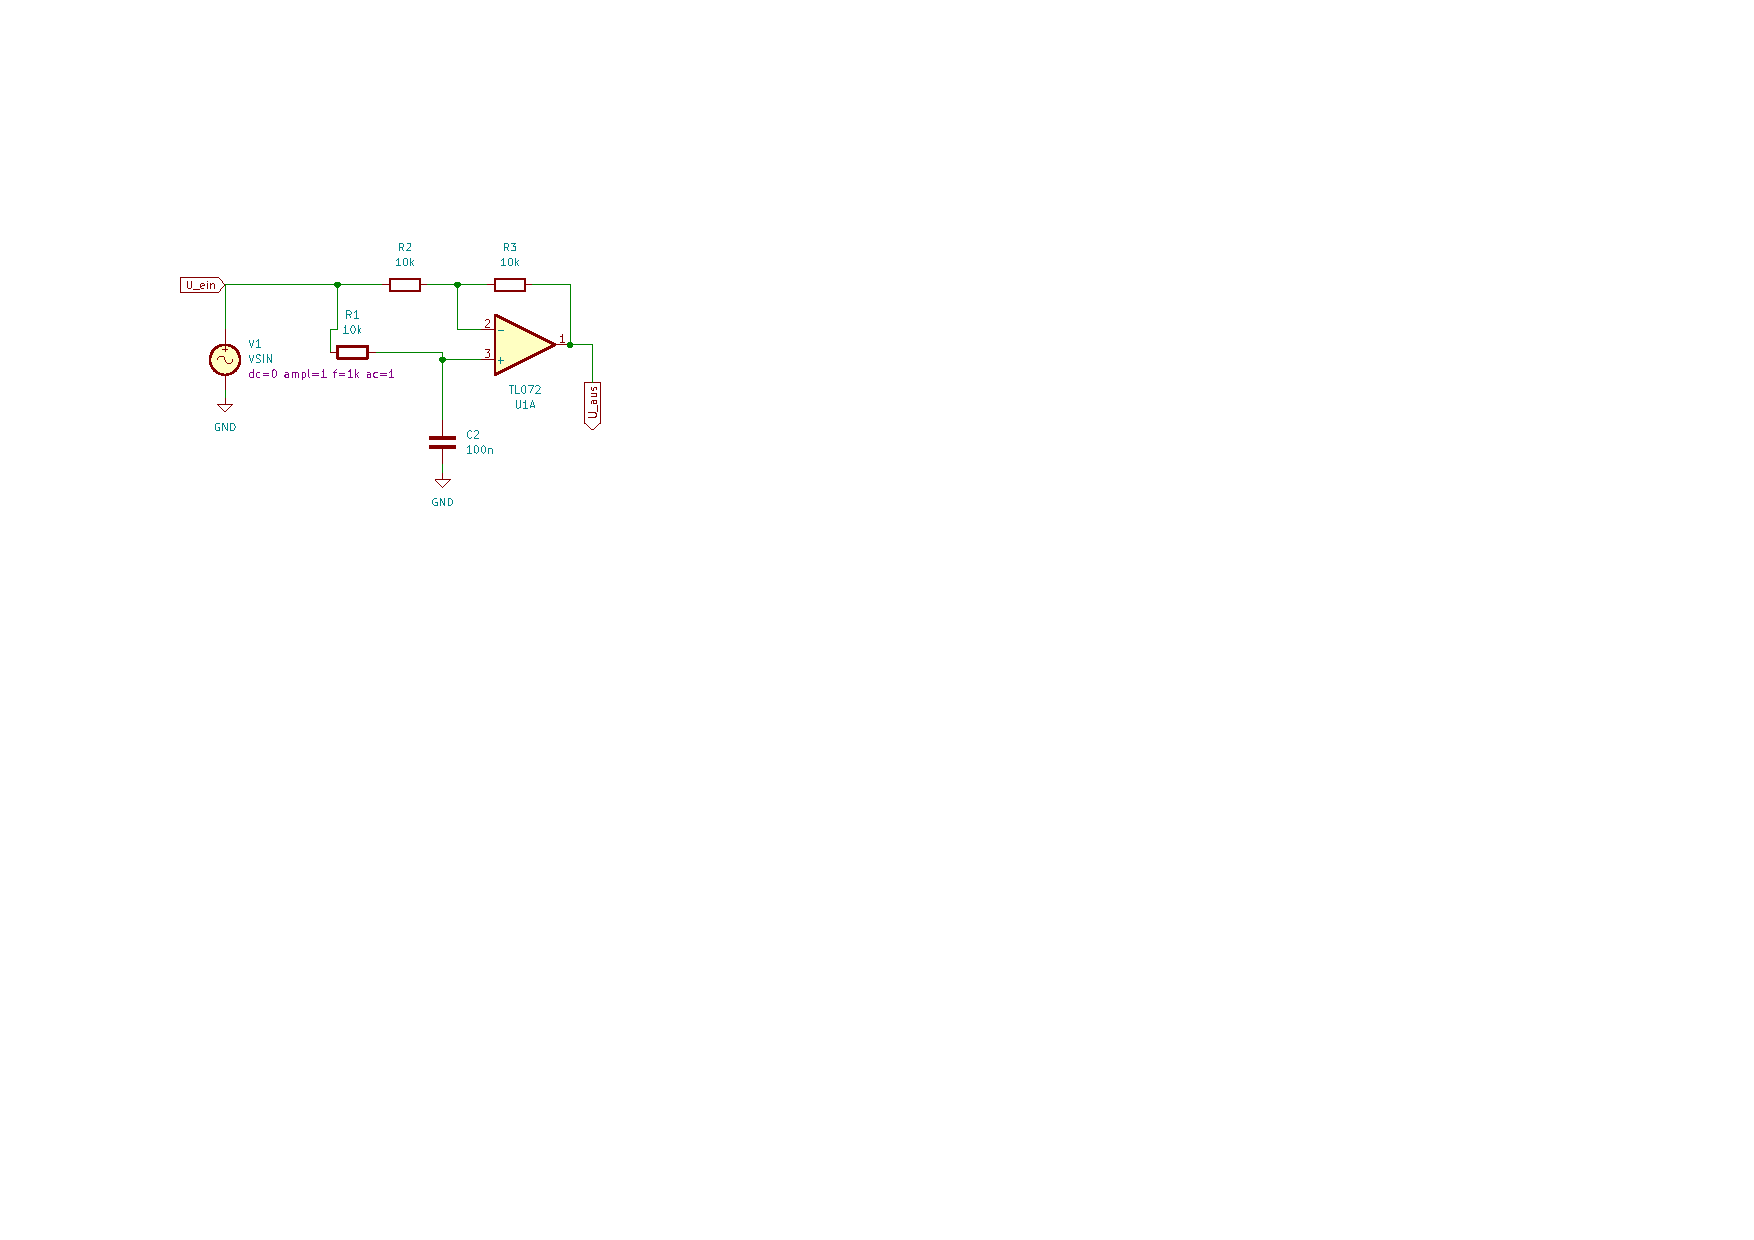
\includegraphics[width=0.7\linewidth]{Elektronik-Laborprotokoll_Filter/Circuits/allpas_circuit.pdf}
 \caption{ Allpassfilter-Schaltung}
 \label{fig:Allpass_circuit}
\end{figure}
%
Dann wurde ein Bessel-Tiefpass 3.Ordnung(Gain 9, $f_g=\SI{500}{\hertz}$  mithilfe des Filter Design Tool vom Texas Instruments \cite{Texas_Instruments} dimensioniert(\ref{fig:Bessel_Tiefpass_3.Ordnung}).
%
\begin{figure}[H]
 \centering
 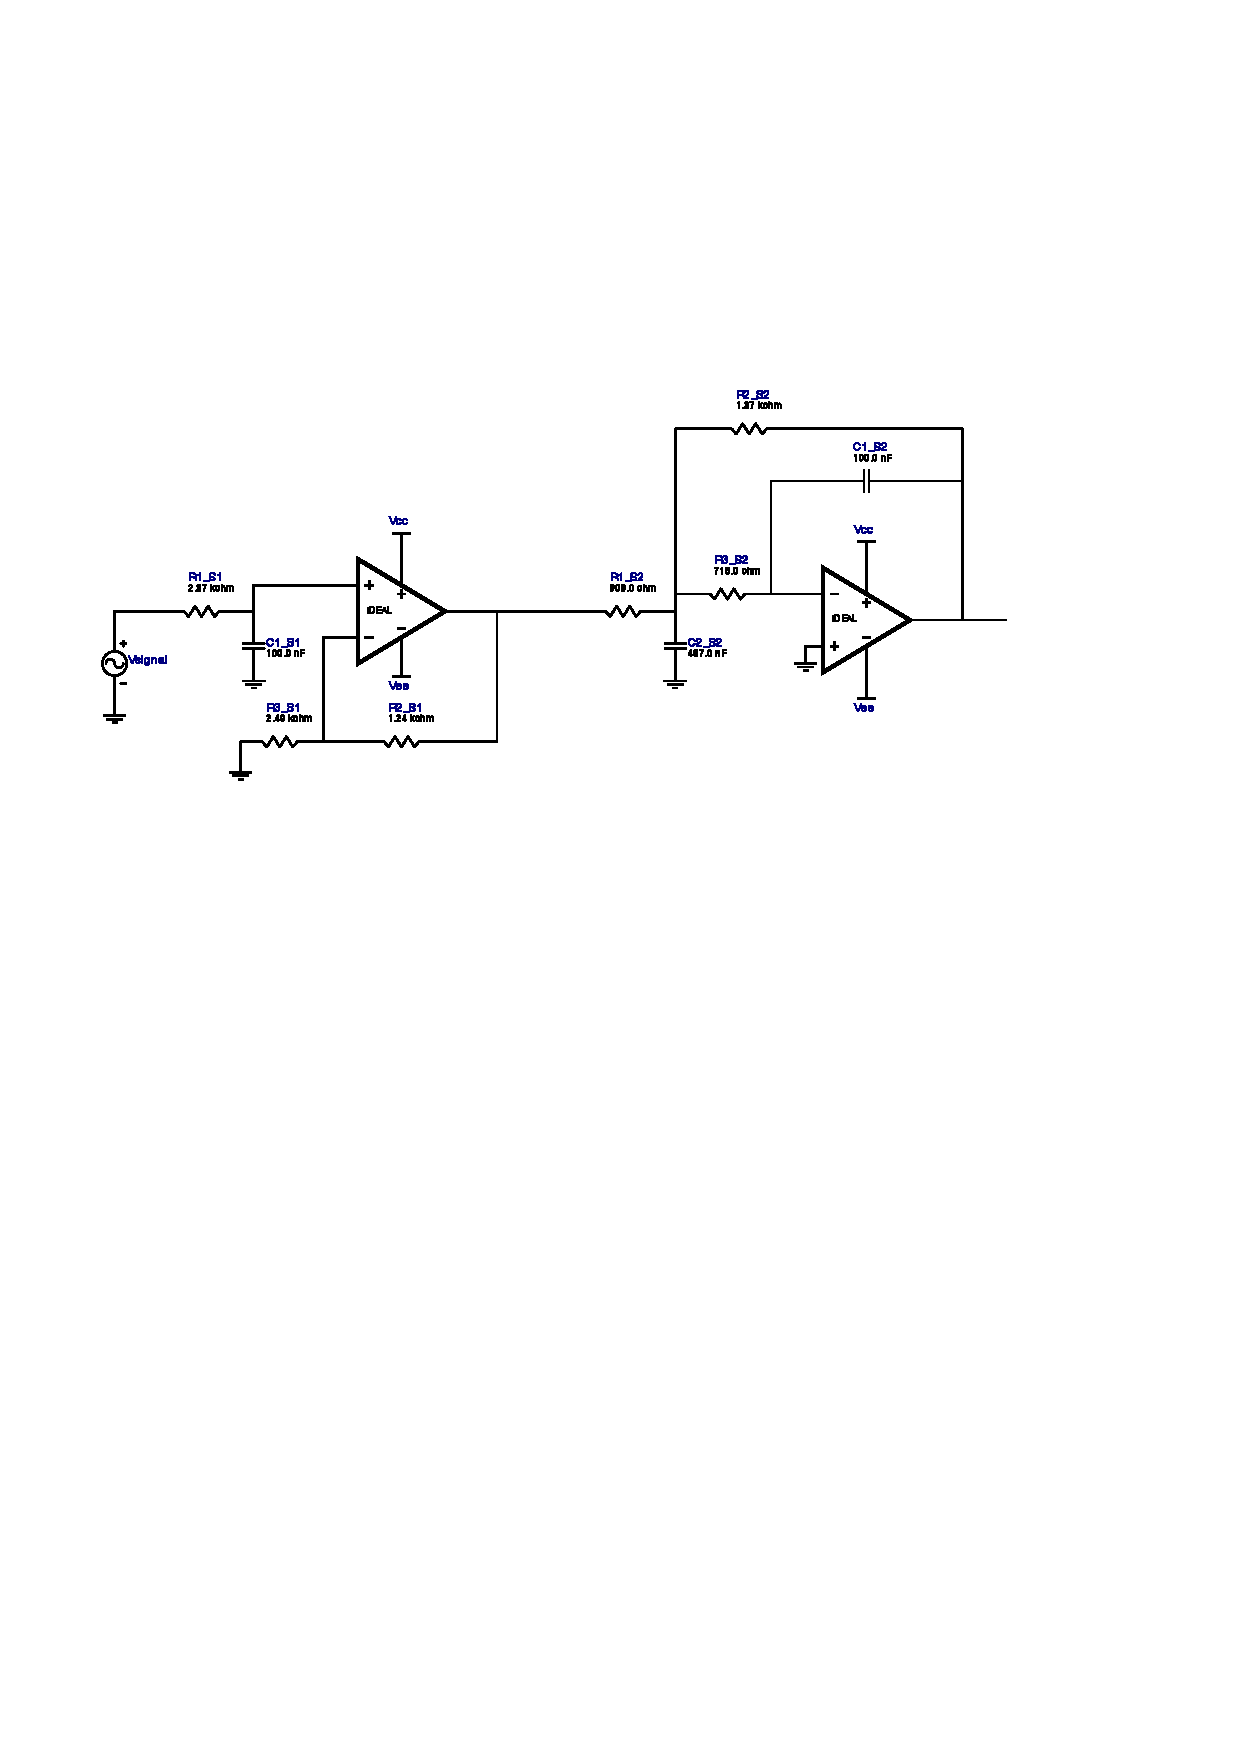
\includegraphics[width=0.7\linewidth]{Elektronik-Laborprotokoll_Filter/Circuits/Bessel_3.Ordnung_Filter_Tool.pdf}
 \caption{ Bessel-Tiefpass 3.Ordnung -Schaltung}
 \label{fig:Bessel_Tiefpass_3.Ordnung}
\end{figure}
%
Die Bessel-Tiefpass 3.Ordnung wurde simuliert und dann mithilfe einem Lag-Kompensator erweitert \ref{fig:Bessel_Tiefpass_3.Ordnung_Kompensiert}. 


\begin{figure}[H]
 \centering
 \includegraphics[width=0.7\linewidth]{Elektronik-Laborprotokoll_Filter/Circuits/tiefpass3besselpluslagpass_circuiıt.pdf}
 \caption{ Bessel-Tiefpass 3.Ordnung -Schaltung}
 \label{fig:Bessel_Tiefpass_3.Ordnung_Kompensiert}
\end{figure}

Für das Bodediagramm benötigte Messdaten wurden sowohl für die Schaltung ohne als auch mit dem Kompensator aufgenommen.




%Die Universalfilter-Schaltung ermöglicht die Erzeugung von Tiefpass-, Bandpass- und Hochpasssignalen. Tief- und Hochpassfilter sind dabei 2. Ordnung, während der Bandpass ein Filter 1. Ordnung ist. Diese Filter sind besonders interessant, da die individuellen Filterparameter leicht verändert werden können, ohne dass ein Parameter die anderen beeinflusst. Daher finden solche Filter beispielsweise Anwendung in vollparametrischen Equalizern, bei denen Verstärkung, Frequenz und Bandbreite unabhängig voneinander eingestellt werden können. Die Schaltung für ein Universalfilter, auch als variable State Filter bezeichnet, besteht aus zwei Integratoren und einem Differenzverstärker.Der erste Integrator bekommt sein Eingangssignal vom Ausgang des Differenz-Verstärkers, welches das Hochpass Signal ist, und gibt sein Ausgangssignal an den nächsten Integrator, sowie an den nicht-invertierenden Eingang des Differenz-Verstärkers. Dieses Signal ist das Bandpass Signal. Das Ausgangssignal des zweiten Integrators stellt den Tiefpass Ausgangdar und ist mit dem invertierenden Eingang des Differenz-Verstärkers verbunden, ebenso wie das Eingangssignal.






%Notizen (Bitte nicht löschen)
%
%3.2.1: Integrator
%
%benutzt wurde R1= 1MOhm
%
%Parallel zu Kondensator 56Ohm
%
%C=100nF
%
%1.Messung:
%
%10Hz
%1 volt
%
%Ue= 0,469
%Ua= 6,35
%Eingang-Ausgang
%Phasenunterschied =101,7 Grad


%100Hz

%0,469
%Ua= 0,734
%Phase = 90,23

%Betrag
%20*log(U_a/U_e)

%1000Hz
%
%Ue=0,497
%Ua=0.078
%Phase=90,52

%1MGHZ mit 10V gespeichert

%Offset war in der Realität nicht gleich 0.
%Wenn wir den Offset z.B. 0.001 integrieren, dann %sehen wir den Effekt davon.


%Aktive Filter erster Ordnung
%************************

%Tiefpass

%Unser tiefpass ist invertierend.

%Wir können eventuelle Werte invertieren

%Vpp=1V

%10Hz 
%100 Hz 
%160 Hz
%1000Hz
%10kHz
%100kHz
%500kHz

%Beide Widerstände 10KOhm



%Für Tiefpassfilter haben wir mit Oszillloskop am %COmputer 
%Bodediagramm gespeichert




%PI FILTEr:


%Für Sprungantwort wurde eingestellt
%Form:Rechteckspannung
%Frequenz 100Hz
%(Periode 10ms)
%Amplitude 1Volt
%Offset 1Volt
%alpha=50\%


%Hochpasssverhalten bei eiener Frequenz höher als 10kHz liegt an dem OPV selbst an.
%Das kann nicht mit der externen Schaltung erklärt werden.

